\documentclass[12pt, a4paper]{article}
\usepackage[a4paper, includeheadfoot, mag=1000, left=2cm, right=1.5cm, top=1.5cm, bottom=1.5cm, headsep=0.8cm, footskip=0.8cm]{geometry}

% Fonts
\usepackage{fontspec, unicode-math}
\setmainfont[Ligatures=TeX]{PT Serif}
\setmonofont{CMU Typewriter Text}
\usepackage[english, russian]{babel}

% Indent first paragraph
\usepackage{indentfirst}
\setlength{\parskip}{5pt}

% Diagrams
\usepackage{graphicx}
\usepackage{float}
\usepackage{subcaption}

% Page headings
\usepackage{fancyhdr}
\pagestyle{fancy}
\renewcommand{\headrulewidth}{0pt}
\setlength{\headheight}{16pt}

% new font       name                fontname in system
% \newfontfamily\namefont[Scale=1.2]{Gloria Hallelujah}
\fancyhead{}

% Use case template
\usepackage{xifthen}
\newcommand{\uctitle}[1]{\renewcommand{\givenuctitle}{#1}}
\newcommand{\givenuctitle}{Не указано}
\newcommand{\ucgoal}[1]{\renewcommand{\givenucgoal}{#1}}
\newcommand{\givenucgoal}{Не указано}
\newcommand{\ucscenario}[1]{\renewcommand{\givenucscenario}{#1}}
\newcommand{\givenucscenario}{}
\newcommand{\ucextensions}[1]{\renewcommand{\givenucextensions}{#1}}
\newcommand{\givenucextensions}{}
\newenvironment{usecase}{}{
  \noindent\fbox{
    \parbox{0.98\textwidth}{
      \vspace{2mm}
      \textbf{\large \givenuctitle}\\[3mm]
      \textbf{Цель:} \givenucgoal\\[2mm]
      \textbf{Сценарий:}
      \begin{enumerate}\givenucscenario\end{enumerate}
      \textbf{Расширения:}
      \begin{itemize}\givenucextensions\end{itemize}
    }
  }
}
\newenvironment{usecasenoext}{}{
  \noindent\fbox{
    \parbox{0.98\textwidth}{
      \vspace{2mm}
      \textbf{\large \givenuctitle}\\[3mm]
      \textbf{Цель:} \givenucgoal\\[2mm]
      \textbf{Сценарий:}
      \begin{enumerate}\givenucscenario\end{enumerate}
    }
  }
}

\begin{document}

% Title page
\begin{titlepage}
\begin{center}

\textsc{«УНИВЕРСИТЕТ ИТМО»\\[4mm]
Кафедра вычислительной техники}
\vfill
\textbf{КУРСОВАЯ РАБОТА}\\[4mm]
по дисциплине:\\[2mm]
\textbf{Программирование интернет-приложений}\\[16mm]
\end{center}

\begin{flushright}
Выполнили: \\[4mm]
Калугина Марина Максимовна \\[2mm]
Каюков Иван Алексеевич \\[2mm]
Группа P3202
\end{flushright}

\begin{center}
\vfill
Санкт-Петербург\\[2mm]
2018 г.

\end{center}
\end{titlepage}


\begin{center}
\textsc{Darknet RoboGit \&\& RoboStore}
\vspace{12mm}
\end{center}
\tableofcontents
\newpage

% Contents

\section{О проекте}

Предметом разработки является \textit{RoboGit} -- платформа для хостинга 
робототехнических проектов, который основан на системе контроля версий
\textit{Git} с поддержкой \textit{markdown} и \textit{RoboStore} -- интернет-магазин
с товарами для робототехники на домене \textit{.onion}, поддерживающий
оплату криптовалютой.
Платформа позволяет пользователям формировать заказ на покупку
необходимого для текущего проекта комплекта деталей и совершать покупку
необходимого в один клик.

\subsection{Цель создания}

\begin{itemize}
\item Предоставляние пользователям возможности размещения 
  робототехнических проектов и организации пользовательских проектов
  с помощью системы контроля версий \textit{Git}.
\item Поддержание анонимности пользователей.
\item Организация интернет-магазина с товарами для робототехники.
\item Предоставляние пользователям возможности упрощенно совершать покупку
  необходимых для проекта товаров.
\end{itemize}

\subsection{Целевая аудитория}

Плохие парни.

\subsection{Описание прецедентов}

\begin{usecase}
\uctitle{Регистрация и авторизация}
\ucgoal{Завести аккаунт в cистеме, создать пользователь}
\ucscenario{
  \item Незарегистрированный/неавторизироанный пользователь имеет 
    доступ ко всем страницам платформы, кроме своего профиля и 
    создания нового репозитория.
  \item При попытке перейти к себе в профиль (главную страницу
    \textit{RoboGit}) или при попытке создания нового репозитория
    открывается форма авторизации с ссылкой на форму регистрации.
  \item Пользователь автооризируется или переходит на страницу регистрации,
    заполняет поля и отправляет форму.
  \item Система перенаправляет на страницу личного профиля пользователя.
}
\ucextensions{
  \item Ошибка при авторизации (неверный логин/пароль) или ошибка 
    при регистрации (адрес электронной почты уже используется, 
    пароль слишком короткий) предотвращает переход на страницу
    личного профиля.
}
\end{usecase}

\begin{usecase}
\uctitle{Создание нового репозитория}
\ucgoal{Создать новый репозиторий}
\ucscenario{
  \item Авторизированный пользователь переходит на страницу содания 
    нового репозитория.
  \item Открывается форма для ввода имени репозитория и его описания.
  \item После успешной отправки формы появляется страница, в которой 
    описывается как создать репозиторий с командной строки или
    импортировать код.
}
\ucextensions{
  \item Ошибка при создании репозитория (репозиторий уже с таким именем уже
    существует в данном аккаунте) предотвращает создание репозитория.
}
\end{usecase}

\begin{usecasenoext}
\uctitle{Работа с существующим репозиторием}
  \ucgoal{Держать актуальные версии проектов в \textit{RoboGit}.}
\ucscenario{
  \item Работа с существующим репозиторием ведется через командную строку
    пользовательского персонального компьютера.
}
\end{usecasenoext}

\begin{usecase}
\uctitle{Просмотр пользовательских репозиториев}
\ucgoal{Просмотр пользователями репозиториев других пользователей,
  знакомство с кодом и описаниями.}
\ucscenario{
  \item Пользователь открывает страницу репозитория.
  \item Платформа предоставляет обзор всех файлов, находящихся в
    репозитории.
  \item Файлы, написанные при помощи языка разметки \textit{Markdown}
    и имеющие расширение \textit{.md}, представляются на платформе в 
    виде страницы-публикации.
}
\ucextensions{
\item В файлах с расширением \textit{.md} можно указывать товары из
  \textit{RoboStore} для добавления из в корзины пользователей.
}
\end{usecase}

\begin{usecase}
\uctitle{Оценка пользовательских репозиториев}
\ucgoal{Поощрение интересных проектов, создание топа лучших проектов 
  \textit{RoboGit}.}
\ucscenario{
  \item Пользователь отмечает понравившиеся репозитории, нажимая
    кнопку \textit{stars} на странице репозитория.
  \item Система сохраняет информацию о количестве \textit{stars}
    для текущего репозитория.
}
\ucextensions{
\item Параметр \textit{stars} влияет на положение репозитория в топе.
  \item В пользовательских профилях для каждого репозитория
    отображается количество \textit{stars}.
}
\end{usecase}

\begin{usecasenoext}
\uctitle{Формирование заказа на покупку из пользовательских проектов}
\ucgoal{Добавление товара из проекта в корзину в один клик для 
  дальнейшей покупки.}
\ucscenario{
\item Пользователь открывает файл с расширением \textit{.md}, в котором
  есть товар из \textit{RoboStore}.
  \item При нажатии на наименование товара, он отправляется в 
    пользовательскую корзину.
}
\end{usecasenoext}

\begin{usecasenoext}
\uctitle{Просмотр профиля пользователей}
\ucgoal{Просмотр пользовательских профилей, знакомство с репозиториями 
  пользователя.}
\ucscenario{
  \item Пользователь открывает страницу пользовательского профиля.
  \item Платформа предоставляет обзор всех репозиториев пользователя.
}
\end{usecasenoext}

\begin{usecasenoext}
\uctitle{Просмотр главной страницы магазина}
\ucgoal{Ознакомить пользователей с асортиментом магазина.}
\ucscenario{
  \item Главная страница платформы содержит краткое описание товара.
  \item Пользователь имеет возможность выбрать категорию товара, при выборе
    категории на странице остаются товары только выбранной категории.
  \item Платформа позволяет отфильтровать товары. Фильтры для каждой
    категории товаров индивидуальны.
}
\end{usecasenoext}

\begin{usecasenoext}
\uctitle{Просмотр страницы товара}
\ucgoal{Позволяет пользователем подробнее ознакомиться с товаром.}
\ucscenario{
  \item С краткого описания товара на главной странице \textit{RoboStore} 
    пользователь может перейти к просмотру страницы товара, нажав на 
    кнопку "Подробнее".
  \item После нажатия кнопки пользователь переходит на страницу с подробным
    описанием товара (характеристики, описание).
}
\end{usecasenoext}

\begin{usecasenoext}
\uctitle{Выбор фильтров для товаров}
\ucgoal{Позволить пользователям фильтровать товар по характеристикам,
  зависящим от категории товара.}
\ucscenario{
  \item После выбора категории товаров, пользователю становится доступен 
    выбор категорий для фильтров товаров.
  \item Пользователь может установить необходмые ему фильтры и
    отправить форму.
  \item После отправки формы платформа оставит товары, удовлетворяющие 
    фильтру.
}
\end{usecasenoext}

\begin{usecasenoext}
\uctitle{Добавление товаров в корзину}
\ucgoal{Формирование пользовательской корзины для дальнейшего 
  оформления заказа.}
\ucscenario{
  \item С краткого описания товара на главной стронице \textit{RoboStore}
    пользователь может перейти к просмотру страницы товара, нажав на
    кнопку "В корзину".
  \item После этого платформа отправляет товары пользовательскую корзину.
}
\end{usecasenoext}

\begin{usecase}
\uctitle{Просмотр корзины}
\ucgoal{Ознакомить пользователя с корзиной для дальнейшего формирования
  заказа.}
\ucscenario{
  \item Пользователь открывает страницу с личной корзиной.
  \item В один клик пользователь может изменить количество товаров в заказе,
    удалить товар из корзины или начать оформлять заказ.
}
\ucextensions{
  \item Если корзина пуста, платформа предлагает перейти на главную 
    страницу \textit{RoboStore}.
}
\end{usecase}

\begin{usecasenoext}
\uctitle{Формирование заказа}
\ucgoal{Сформировать заказ для покупки товара.}
\ucscenario{
  \item Пользователь нажимает кнопку формирования товара.
  \item Открывается страница, которая предоставляет пользователю ссылку для
    связи с телеграм-ботом для дальнейшего формирования заказа.
}
\end{usecasenoext}

\begin{usecasenoext}
\uctitle{Просмотр лучших проектов}
\ucgoal{Ознакомление с лучшими проектами \textit{RoboGit}.}
\ucscenario{
  \item Система создает топ лучших репозиториев исходя из количества 
    \textit{stars} в пользовательских проектах.
  \item Пользователь может посетить страницу топа лучших репозиториев.
}
\end{usecasenoext}

\begin{usecase}
\uctitle{Добавление товара}
\ucgoal{Поддержание полной базы товаров \textit{RoboStore}.}
\ucscenario{
  \item Сотрудник \textit{Robostore} нажимает кнопку добавление товара 
    в \textit{Robostore}.
  \item Сотрудник заполняет форму с необходимой информацей о товаре.
  \item Сотрудник отправляет форму и публикует товар.
}
\ucextensions{
  \item Если сотрудник не заполняет обязательные поля, система 
    предотвращает публикацию товара в \textit{Robostore}.
}
\end{usecase}

\begin{usecase}
\uctitle{Обновление информации о товаре}
\ucgoal{Поддержание актуальной информации о товарах.}
\ucscenario{
  \item Сотрудник Robostore нажимает кнопку изменения товара 
    в \textit{Robostore}.
  \item Сотрудник получает форму с заполненой ранее информацией 
    о товаре.
  \item Сотрудник изменяет необходимые поля формы.
  \item Сотрудник отправляет форму и система обновляет информацию 
    о товаре.
}
\ucextensions{
  \item Если сотрудник оставляет пустыми обязательные поля, система 
    предотвращает обновление информации о товаре в \textit{Robostore}.
}
\end{usecase}


\begin{usecasenoext}
\uctitle{Удаление товара}
\ucgoal{Удаление неактуальной информации.}
\ucscenario{
  \item Сотрудник \textit{Robostore} нажимает кнопку удаления 
    товара в \textit{Robostore}.
  \item Система удаляет товар.
}
\end{usecasenoext}

\begin{usecasenoext}
\uctitle{Изменение прав пользователей}
\ucgoal{Поддержание актуальной базы сотрудников и администраторов.}
\ucscenario{
  \item Администратор может поменять права пользователя на 
    сотрудника, обычного пользователя или администратора.
  \item Система дает необходимые права пользователю.
}
\end{usecasenoext}

\subsection{UML-диаграмма прецедентов}

\begin{figure}[H]
  \centering
  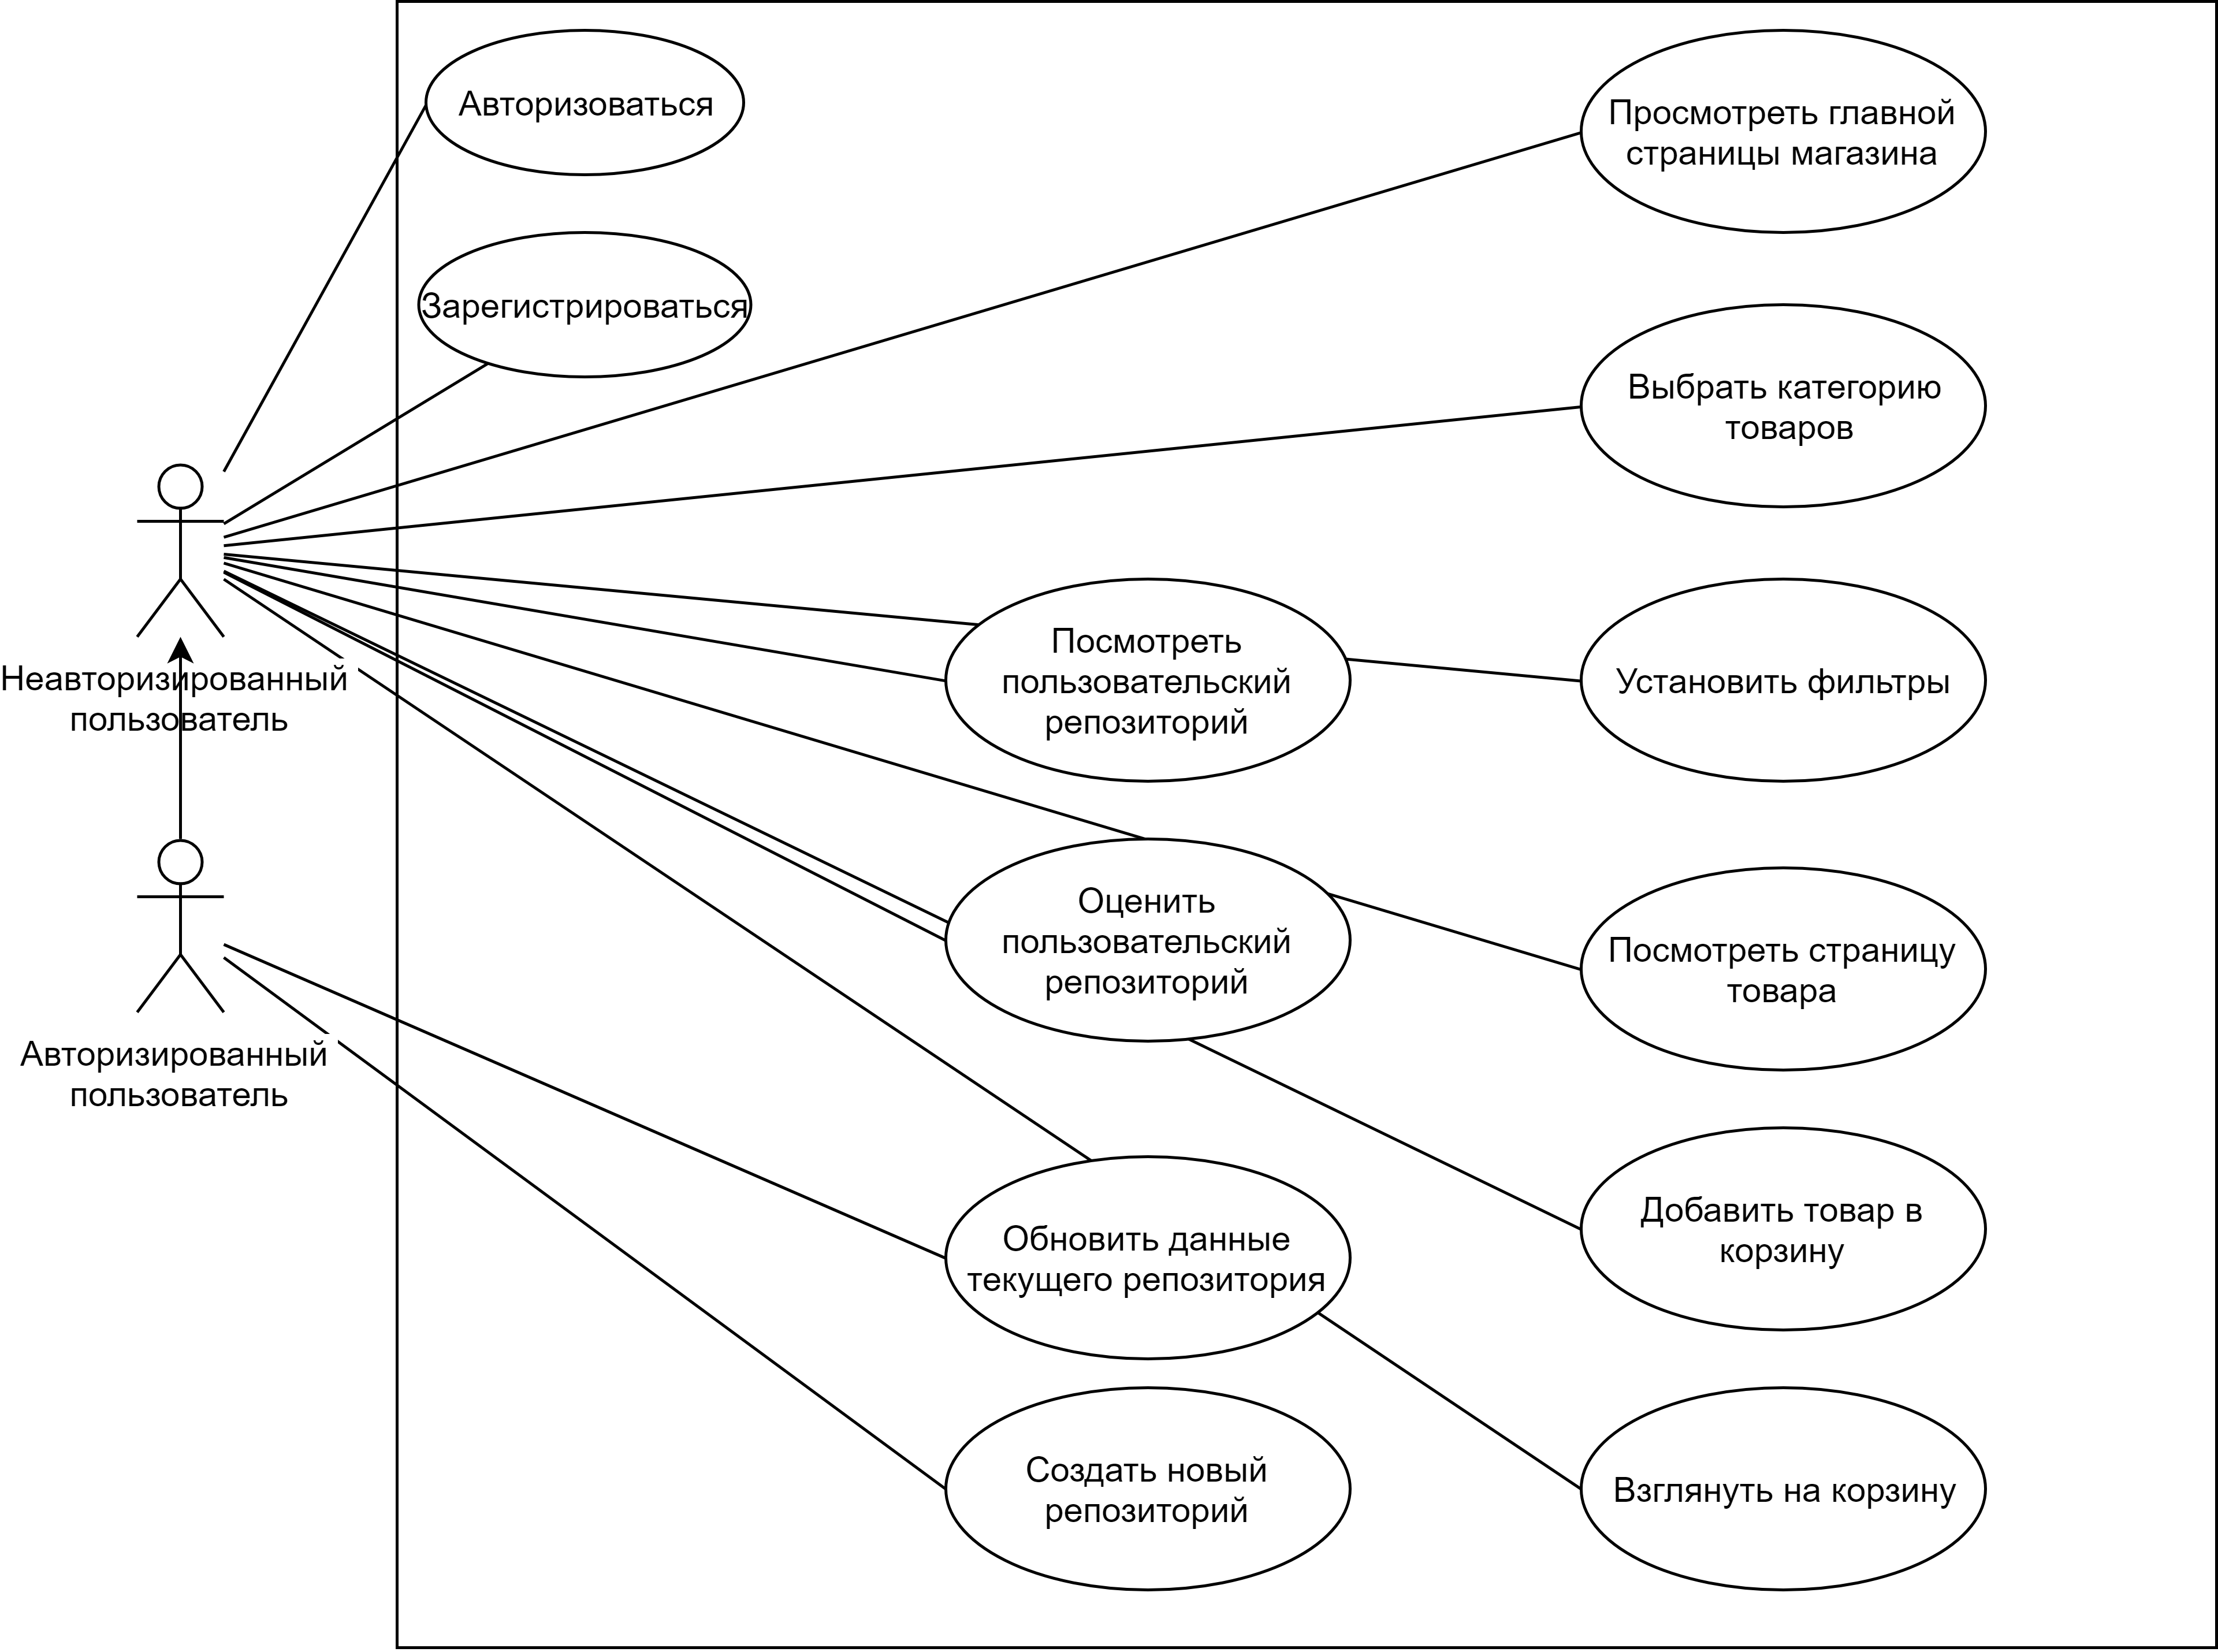
\includegraphics[width=16cm]{uml-precedents.png}
  \caption{UML-диаграмма прецедентов}
\end{figure}

\section{Требования к аппаратно-программному обеспечению}

\subsection{Требования к серверному обеспечению}

Система, которая обеспечивает выполнение программных продуктов сервера 
приложений и хранение данных платформы, должна отвечать следующим требованиям:

\begin{enumerate}
\item Наличие операционной системы \textit{Linux}
\item Наличие сервера ба данных \textit{PostgreSQL} 
  версии 9.6 или выше
\item Наличие сервера приложений \textit{GlassFish} версии
  4.1.2 или выше
\item Наличие на сервере \textit{JDK} 8
\end{enumerate}

\subsection{Требования к клиентскому обеспечению}

Браузерный интерфейс разрабатывается с учетом следующих требований к
программному обеспечению на стороне пользователя:

\begin{enumerate}
\item Веб-браузер \textit{Tor} версии 8.01 или выше
\item Включенный интерпретатор сценариев \textit{JavaScript}.
\item Отсутствие запрета веб-страницам платформы доступа к внешним 
  ресурсам, а именно изображениям, шрифтам, таблицам стилей
  \textit{CSS} и сценариям \textit{JavaScript}, в том числе
  блокировщиками рекламы.
\end{enumerate}

\section{Требования к архитектуре системы}

\subsection{Уровень back-end}

\begin{enumerate}
\item Уровень back-end основывается на \textit{Spring} версии 5
  или выше.
\item Взаимодействие между уровнями back-end и front-end организуется
  посредством \textit{REST API}.
\item Для доступа к БД использeтся \textit{Spring Data}.
\item Серверное приложение должно отправлять пользователям
  еженедельное новостноe сообщение электронной почты,
  используя \textit{JavaMail API}.
\item Серверное приложение должно логировать все вызовы методов 
  на уровне бизнес-логики системы с использованием технологии
  \textit{Spring AOP} и \textit{AspectJ}.
\item Ролевое разграничение доступа к внутренним разделам системы 
  организовано с помощью технологии \textit{Spring Security}.
\item Доступ пользователей в систему осуществляется через систему 
  "единого входа" (Single Sign On). В качестве провайдера SSO использована 
  система \textit{ForgeRock OpenAM}, развёрнутая на отдельном экземпляре 
  (домене) сервера приложений.
\end{enumerate}

\subsection{Уровень front-end}

\begin{enumerate}
\item Уровень front-end строится на \textit{ReactJS + Redux} 
  с использованием \textit{ES6} и \textit{JSX} и набора
  компонентов \textit{Belle}.
\item Веб-интерфейс адаптирован для отображения в трех режимах:
  \begin{itemize}
  \item \textit{Десктопном}: ширина экрана больше 1105px
  \item \textit{Планшетном}: ширина экрана больше 687px и меньше 1105px
  \item \textit{Мобильном}: ширина экрана меньше 687px
  \end{itemize}
\end{enumerate}

\subsection{Telegram-бот}
\label{telegram-bot}

Для сохранения анонимности пользователей оформление заказа происходит
через телеграм-бота.

\begin{enumerate}
\item Telegram-бот отправляет инструкции и ссылку для оплаты заказа.
\item Telegram-бот позволяет определить время и место доставки заказа.
\end{enumerate}

\section{Требования к надежности и безопасности системы}

\begin{enumerate}
\item Серверное приложение должно содержать механизмы защиты от
  уязвимостей, входящих в список \textit{OWASP TOP-10}.
\item Пароли пользователей должны содержать не менее восьми 
  символов и храниться как криптографический хэш.
\end{enumerate}

\section{Архитектура системы}

\begin{figure}[H]
  \centering
  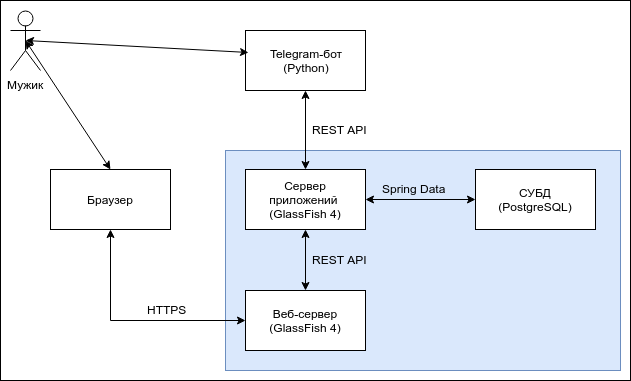
\includegraphics[width=16cm]{system-arch.png}
  \caption{Архитектура системы}
\end{figure}

\section{Функциональные требования}

\subsection{Для неавторизированных пользователей}

\begin{enumerate}
\item Система должна предоставлять пользователю возможность
  зарегистрироваться в системе.
\item Система должна предоставлять пользователям возможность
  авторизоваться с помощью логина и пароля.
\item Система должна предоставлять пользователям возможность
  восстановить пароль.
\item Система должна предостовлять пользователям возможность
  просмотра пользовательских профилей \textit{RoboGit}.
\item Система должна предоставлять пользователям возможность 
  просмора пользовательских репозиториев.
\item Система должна предоставлять возможность пользователям 
  просматривать топ-проектов - пректы, имеющие наибольшее 
  количество \textit{stars}.
\item Система должна предоставлять возможность добавления товара 
  в корзину из пользовательских проектов, выбрав и кликнув на 
    необходимый товар в \textit{markdown} файле.
\item Система должна предоставлять возможность просмотра главной 
  страницы интернет-магазина \textit{RoboStore}, в которой расположены 
  все товары.
\item Система должна позволять выбор категории товаров для просмотра.
\item Система должна позволять пользователю выбирать фильтры для 
  товаров. Возможности фильтра зависят от конкретной категории товара.
\item Система должна предоставлять возможность пользователю 
  просматривать страницы товаров с более подробным описанием.
\item С главной страницы товара или со страницы товара система 
  должна позволять добавлять товар в корзину.
\item Система должна предоставлять возможность просмотра корзины.
\item В пользовательской корзине должно быть возможно изменить 
  количество товара и/или удалить товар.
\item С пользовательской корзины система должна предоставлять 
  возможность оформеления заказа, после чего пользователь получает 
  номер своего заказа и ссылку на телеграм-бота для дальнейшего 
  оформления заказа.
\item Система должна предоставлять возможность экспортировать 
  корзину как внешнюю ссылку, нажав на которую, пользователь 
  заполнит свою корзину товарами из экспортированной корзины.
\end{enumerate}

\subsection{Для авторизированных пользователей}

\begin{enumerate}
\item Система должна позволять авторизированному пользователю 
  создавать новый репозиторий.
\item Система должна позваолять авторизированному пользователю 
  обновлять данные текущего репозитория.
\item Система должна поззволять авторизированному пользователю 
  оценивать пользовательские репозитории, нажимая на кнопку \textit{stars} 
  в пользовательском проекте.
\end{enumerate}

\subsection{Для сотрудников}

\begin{enumerate}
\item Система должна позволять сотруднику добавлять товар в
    \textit{RoboStore}.
\item Система должна позволять сотруднику обновлять информацию 
  о товаре в \textit{Robostore}.
\item Система должна позволять сотруднику удалять товар в 
  \textit{RoboStore}.
\end{enumerate}

\subsection{Для администраторов}

\begin{enumerate}
\item Система должна позволять администратору сделать пользователя 
  сотрудником/администратором (назначить привелегии).
\item Система должна позволять администратору сделать другого 
  администратора/сотрудника обычным пользователем (отнять привелегии).
\end{enumerate}

\section{Прототипы интерфейсов}

\begin{figure}[H]
  \centering
  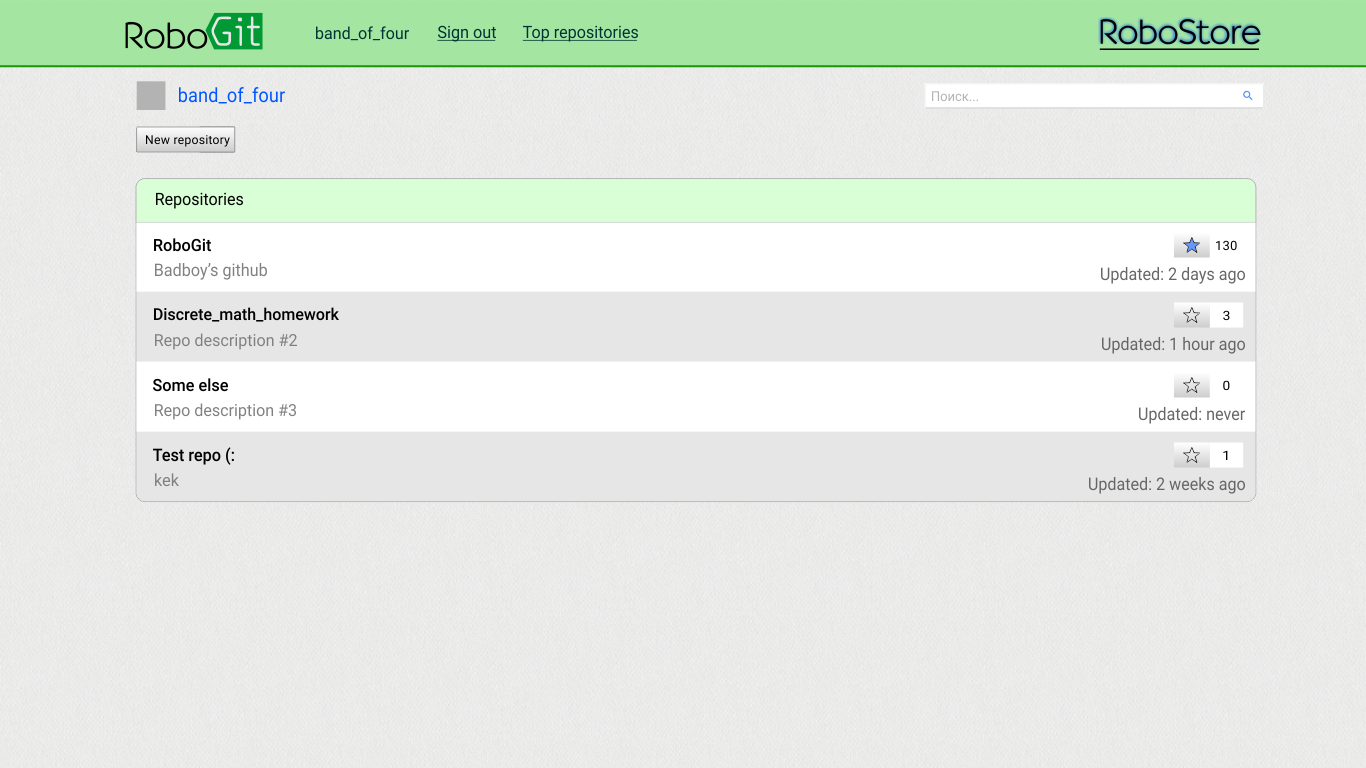
\includegraphics[width=17cm]{png/git_profile.png}
  \caption{Профиль пользователя RoboGit}
\end{figure}

\begin{figure}[H]
  \centering
  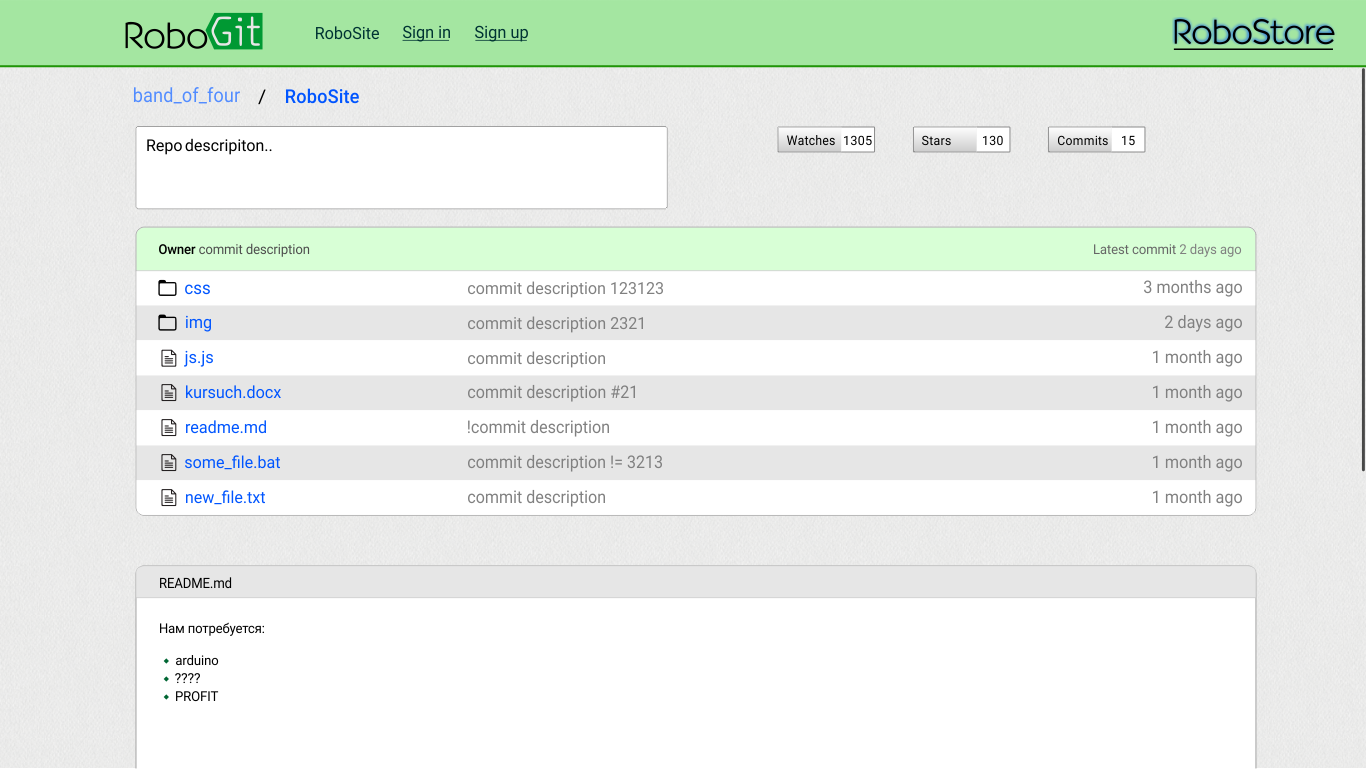
\includegraphics[width=17cm]{png/git_repo.png}
  \caption{Страница репозитория RoboGit}
\end{figure}

\begin{figure}[H]
  \centering
  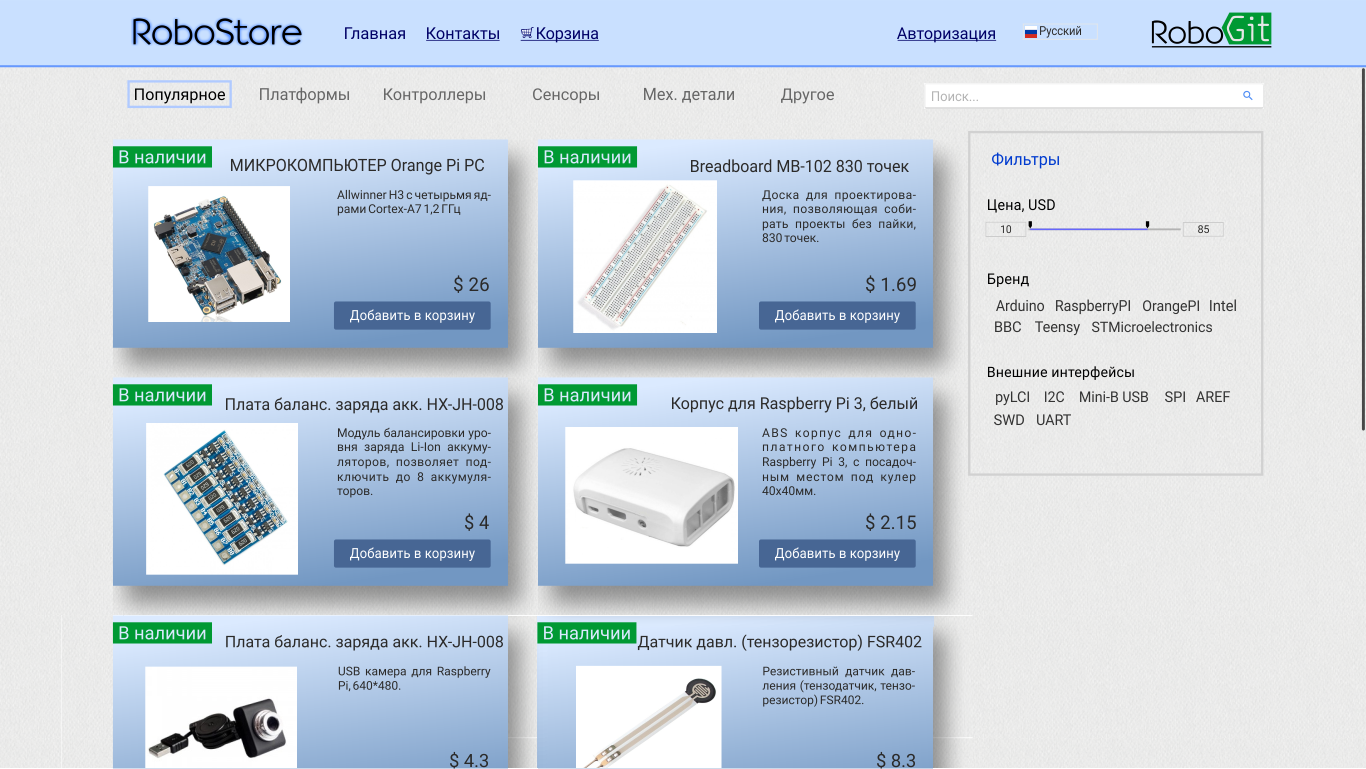
\includegraphics[width=17cm]{png/store_main.png}
  \caption{Главная страница RoboStore}
\end{figure}

\begin{figure}[H]
  \centering
  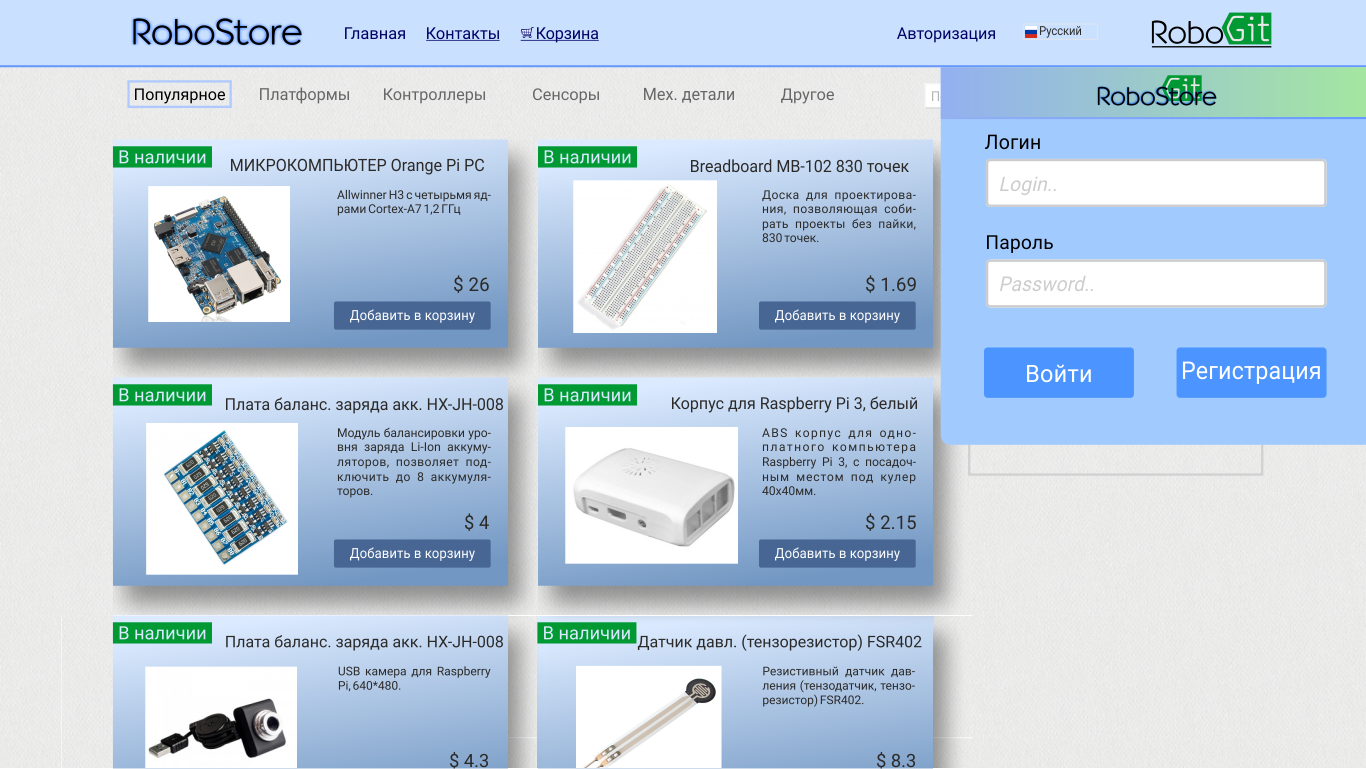
\includegraphics[width=17cm]{png/store_auth.png}
  \caption{Форма авторизации}
\end{figure}

\begin{figure}[H]
  \centering
  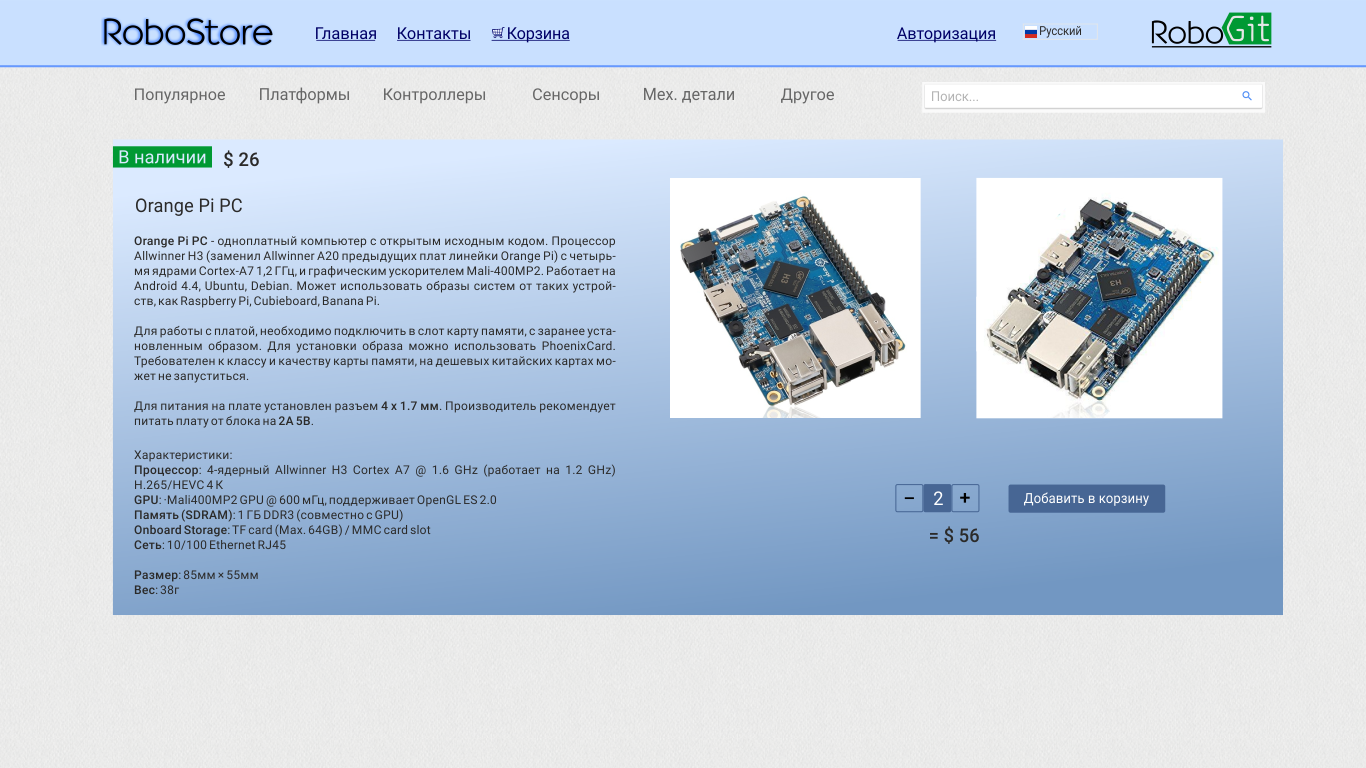
\includegraphics[width=17cm]{png/store_item.png}
  \caption{Страница товара RoboStore}
\end{figure}

\begin{figure}[H]
  \centering
  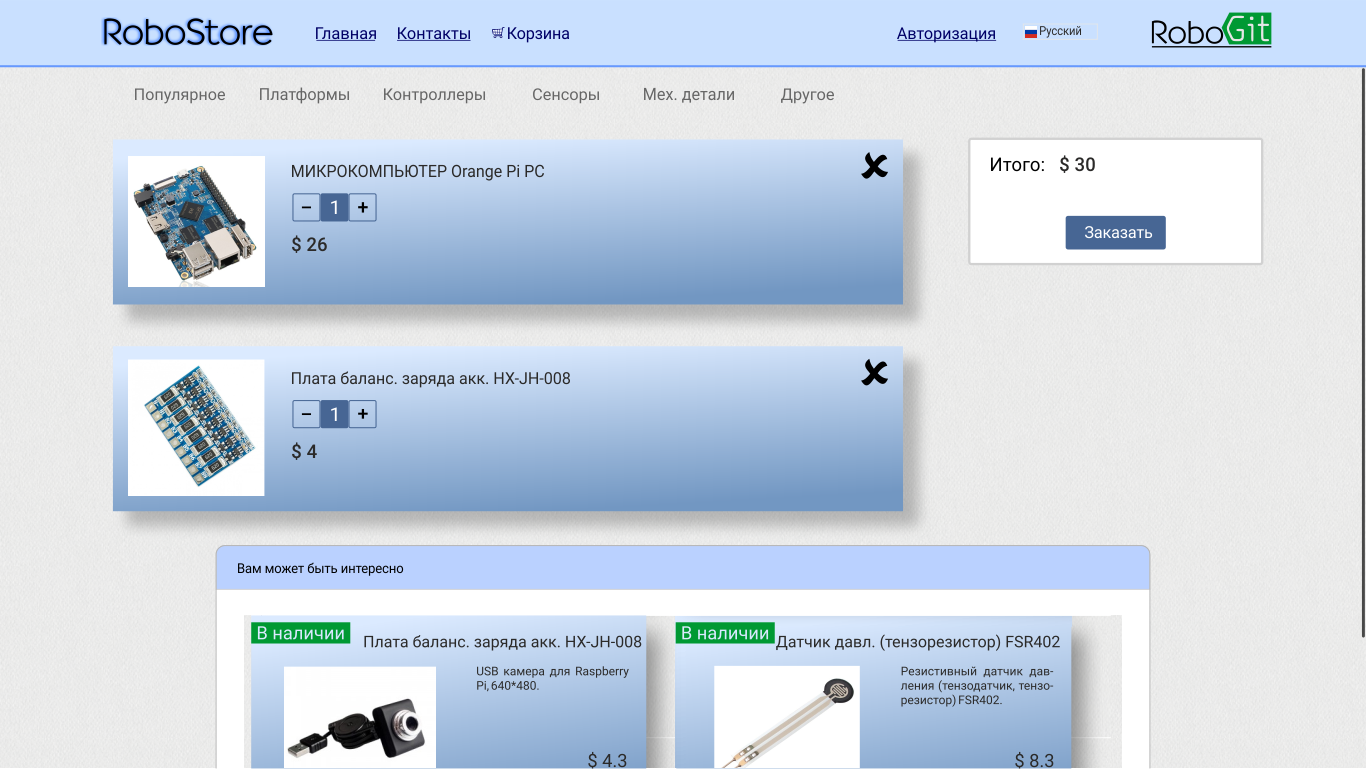
\includegraphics[width=17cm]{png/store_bin.png}
  \caption{Корзина RoboStore}
\end{figure}

\begin{figure}[H]
  \centering
  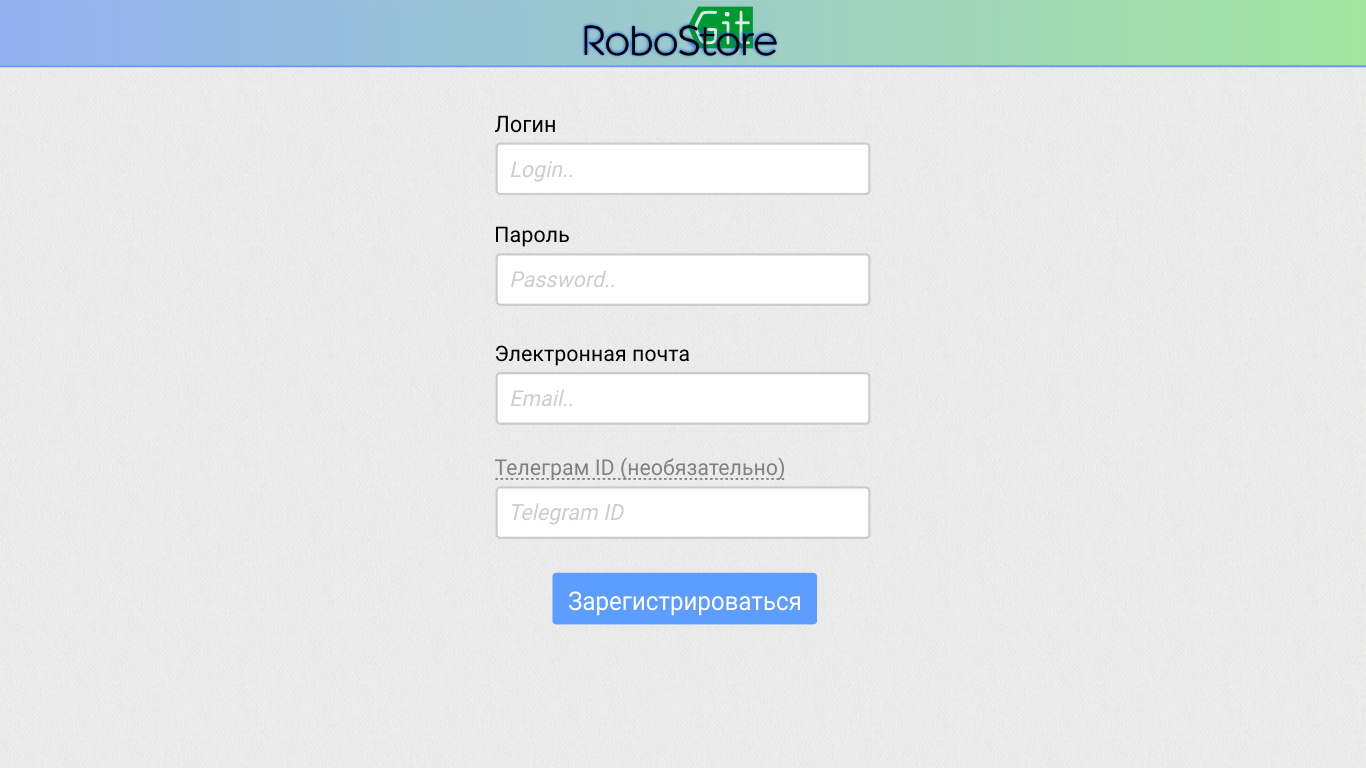
\includegraphics[width=17cm]{png/store_sign.png}
  \caption{Форма регистрации}
\end{figure}

\begin{figure}
  \centering
  \begin{subfigure}[b]{0.47\textwidth}
    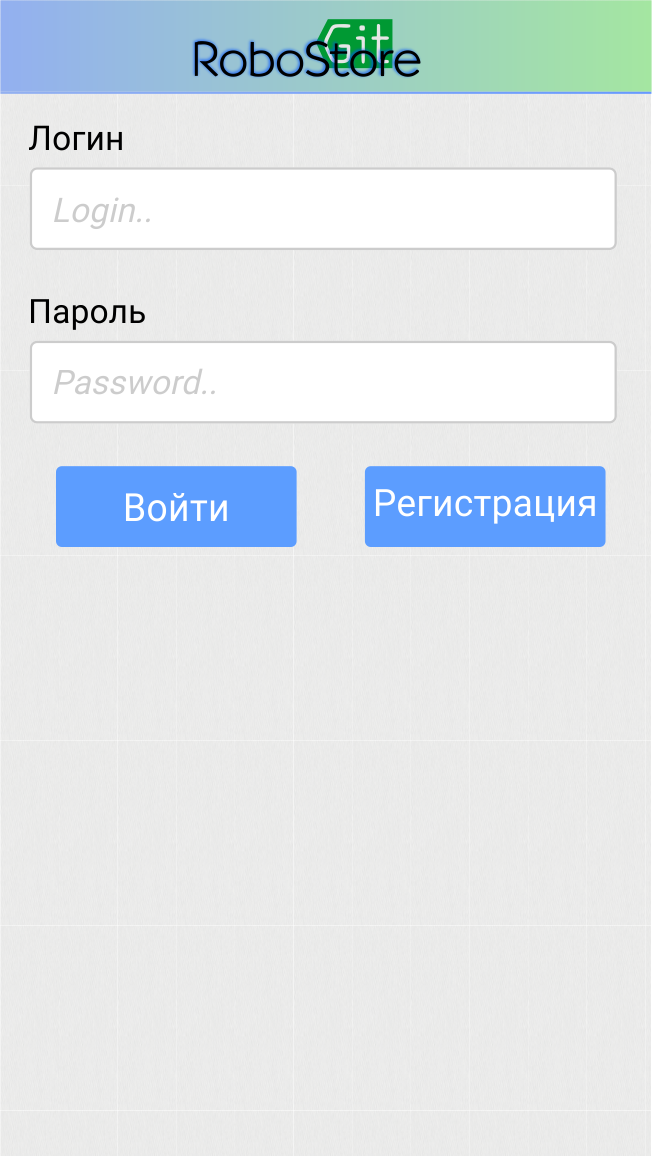
\includegraphics[width=6cm]{png/auth_smart}
    \caption{Форма авторизации}
  \end{subfigure}
  \begin{subfigure}[b]{0.47\textwidth}
    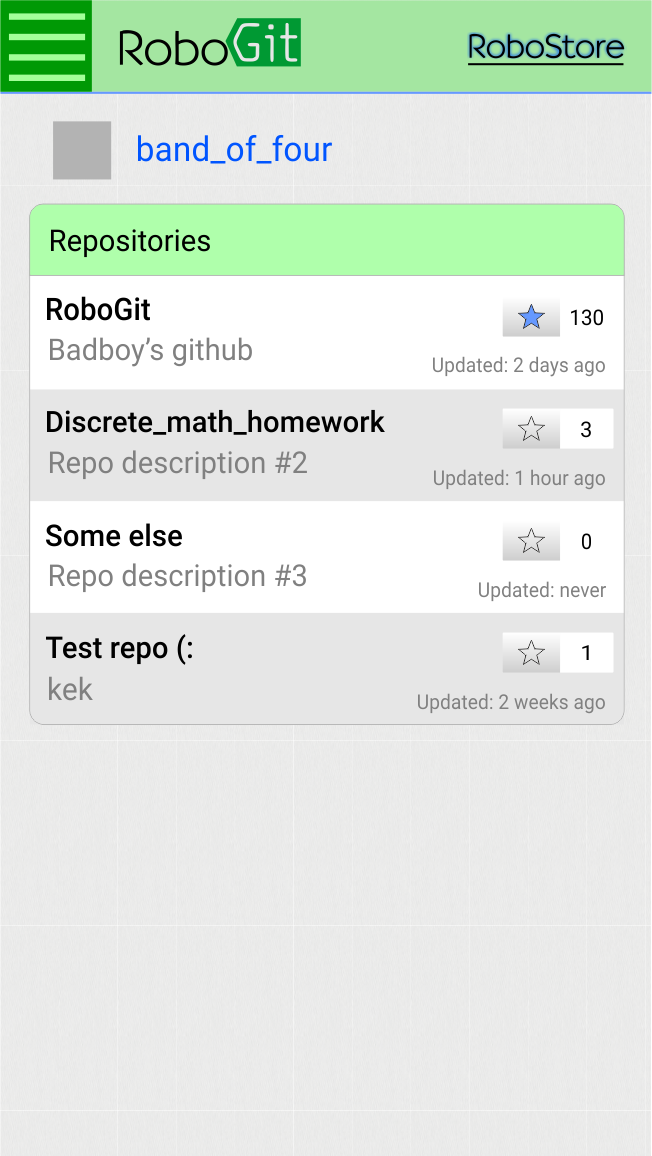
\includegraphics[width=6cm]{png/git_profile_smart.png}
    \caption{Профиль RoboGit}
  \end{subfigure}
  \caption{Макеты для смартфона \textnumero 1}
\end{figure}

\begin{figure}
  \centering
  \begin{subfigure}[b]{0.47\textwidth}
    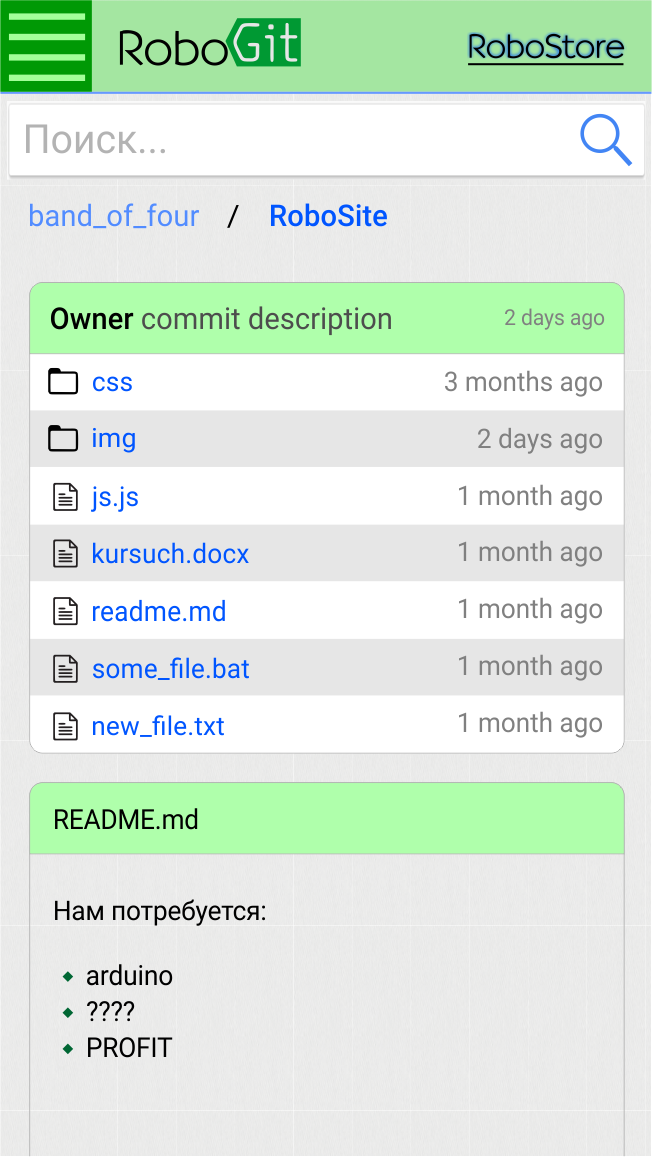
\includegraphics[width=6cm]{png/git_repo_smart.png}
    \caption{Репозиторий RoboGit}
  \end{subfigure}
  \begin{subfigure}[b]{0.47\textwidth}
    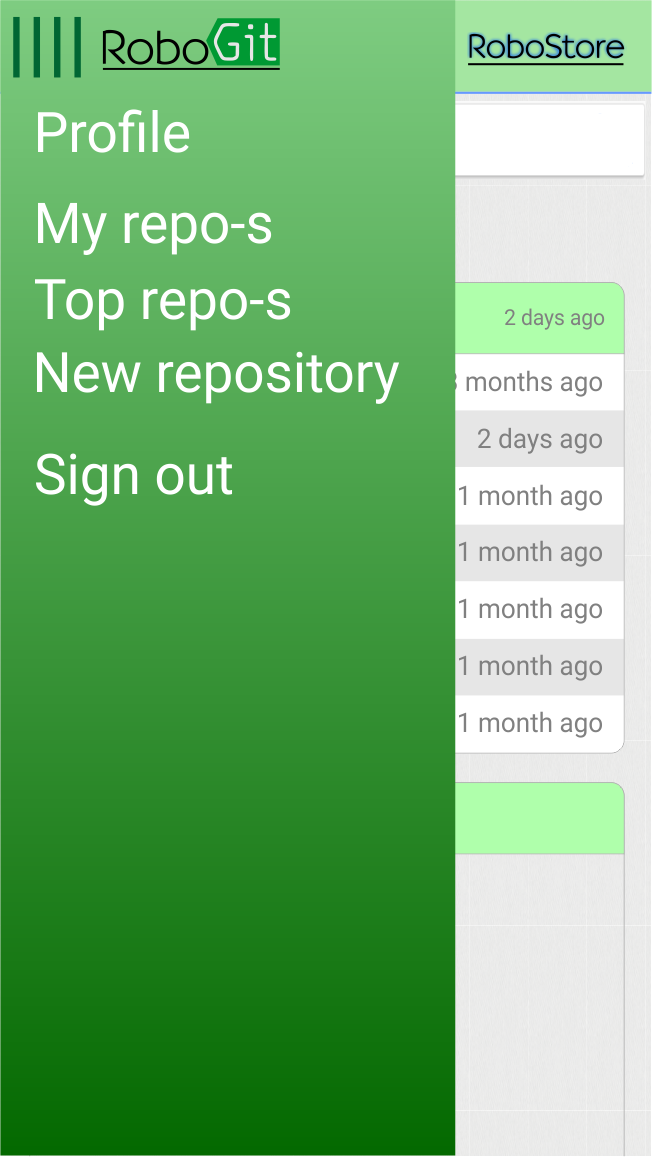
\includegraphics[width=6cm]{png/git_menu_smart.png}
    \caption{Боковое меню RoboGit}
  \end{subfigure}
  \caption{Макеты для смартфона \textnumero 2}
\end{figure}

\begin{figure}
  \centering
  \begin{subfigure}[b]{0.47\textwidth}
    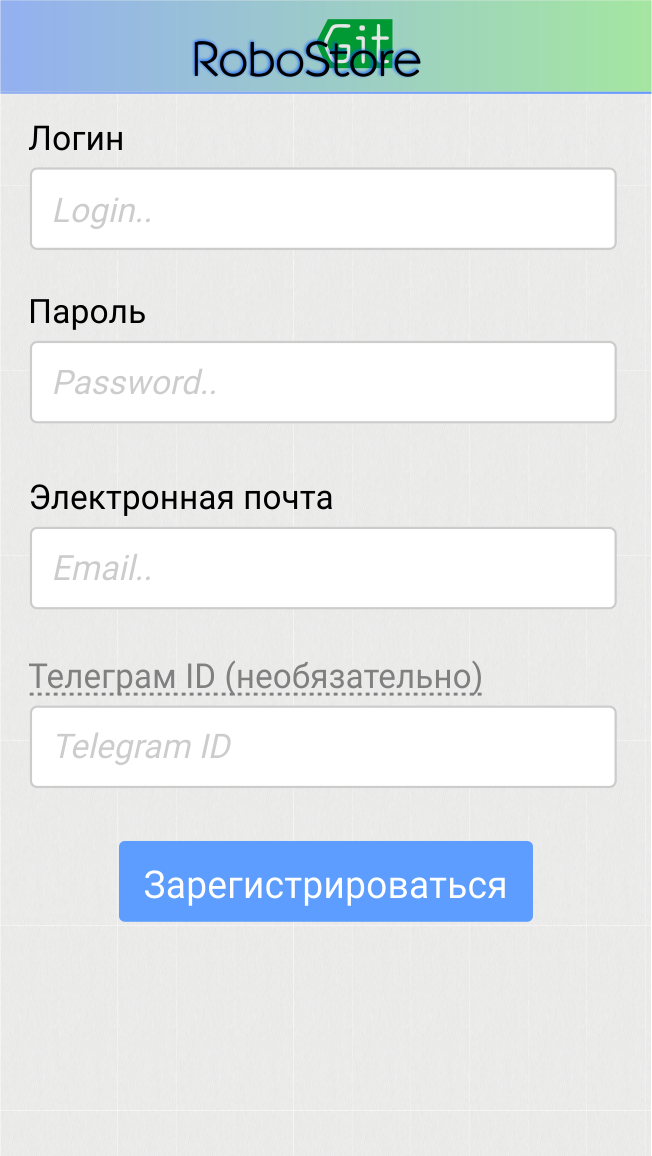
\includegraphics[width=6cm]{png/sign_smart.png}
    \caption{Форма регистрации}
  \end{subfigure}
  \begin{subfigure}[b]{0.47\textwidth}
    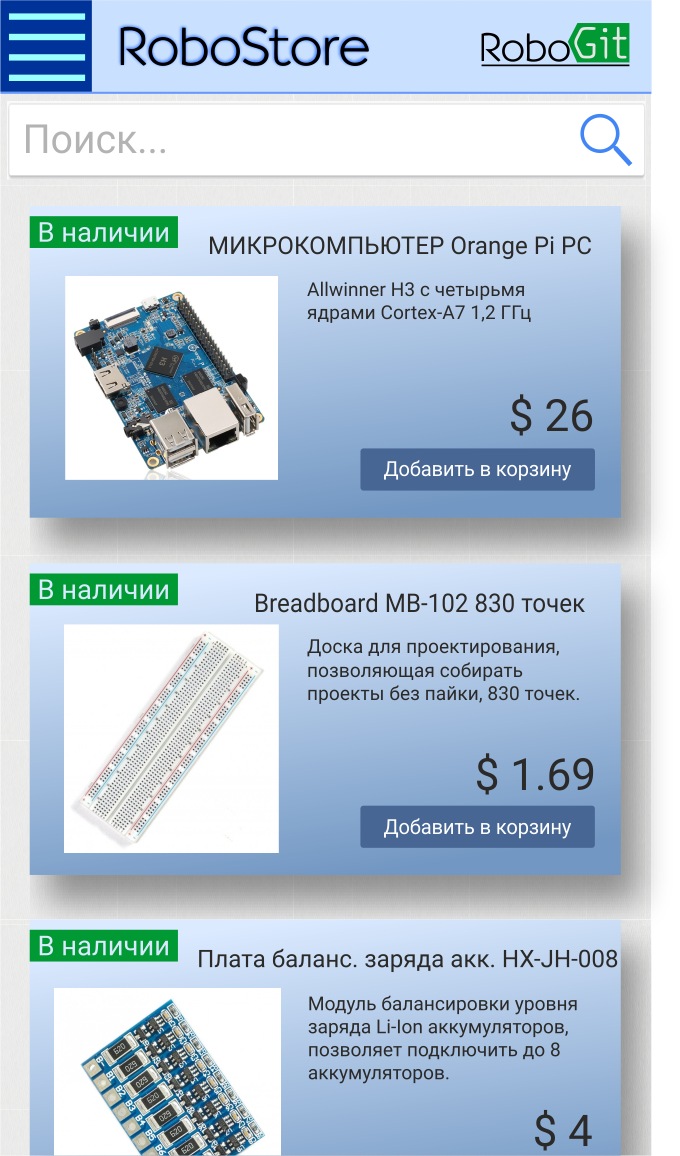
\includegraphics[width=6cm]{png/store_main_smart.png}
    \caption{Главная страница RoboStore}
  \end{subfigure}
  \caption{Макеты для смартфона \textnumero 3}
\end{figure}

\begin{figure}
  \centering
  \begin{subfigure}[b]{0.47\textwidth}
    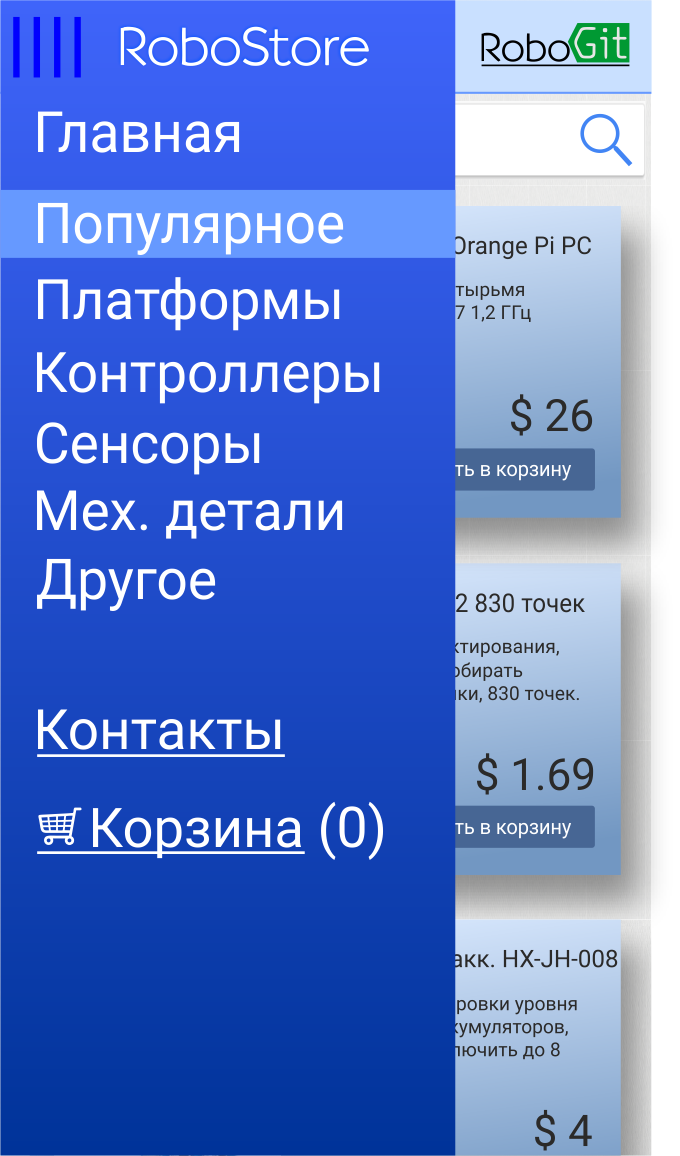
\includegraphics[width=6cm]{png/store_menu_smart.png}
    \caption{Боковое меню RoboStore}
  \end{subfigure}
  \begin{subfigure}[b]{0.47\textwidth}
    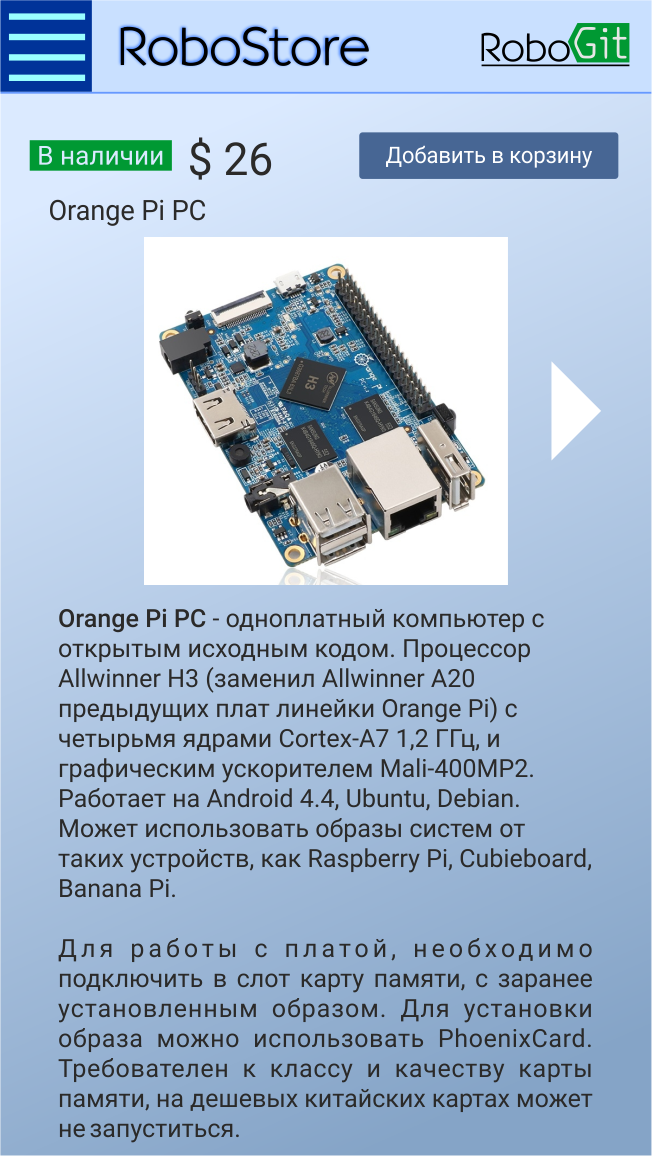
\includegraphics[width=6cm]{png/store_item_smart.png}
    \caption{Страница товара RoboStore}
  \end{subfigure}
  \caption{Макеты для смартфона \textnumero 4}
\end{figure}

\begin{figure}
  \centering
  \begin{subfigure}[b]{0.47\textwidth}
    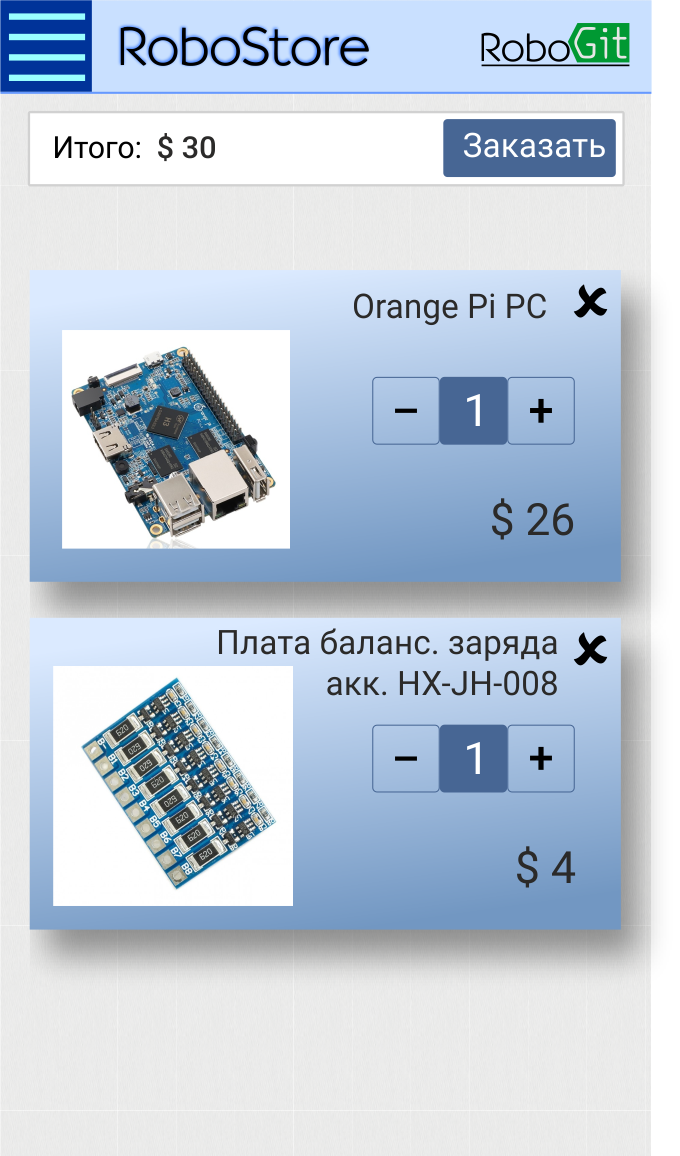
\includegraphics[width=6cm]{png/store_bin_smart.png}
    \caption{Корзина RoboStore}
  \end{subfigure}
  \caption{Макеты для смартфона \textnumero 5}
\end{figure}

\end{document}
